\chapter{Практические задания}

\section*{Задание 1. Написать функцию, которая принимает целое число и возвращает первое четное число, не меньшее аргумента.}

\begin{lstinputlisting}[
	caption={Задание 1},
	label={lst:t1},
	style={lsp},
	linerange={1-4},
	]{../src/main.lsp}
\end{lstinputlisting}

\section*{Задание 2. Написать функцию, которая принимает число и возвращает число того же знака, но с модулем на 1 больше модуля аргумента.}

\begin{lstinputlisting}[
	caption={Задание 2},
	label={lst:t2},
	style={lsp},
	linerange={6-9},
	]{../src/main.lsp}
\end{lstinputlisting}

\section*{Задание 3.  Написать функцию, которая принимает два числа и возвращает список из этих чисел, расположенный по возрастанию.}

\begin{lstinputlisting}[
	caption={Задание 3, вариант 1},
	label={lst:t3-1},
	style={lsp},
	linerange={11-14},
	]{../src/main.lsp}
\end{lstinputlisting}

\begin{lstinputlisting}[
	caption={Задание 3, вариант 2},
	label={lst:t3-2},
	style={lsp},
	linerange={16-17},
	]{../src/main.lsp}
\end{lstinputlisting}

\section*{Задание 4. Написать функцию, которая принимает три числа и возвращает Т только тогда, когда первое число расположено между вторым и третьим.}

\begin{lstinputlisting}[
	caption={Задание 4},
	label={lst:t4},
	style={lsp},
	linerange={19-20},
	]{../src/main.lsp}
\end{lstinputlisting}

\section*{Задание 5. Каков результат вычисления следующих выражений?}

\begin{lstinputlisting}[
	caption={Задание 5},
	label={lst:t5},
	style={lsp},
	linerange={22-27},
	]{../src/main.lsp}
\end{lstinputlisting}

\section*{Задание 6. Написать предикат, который принимает два числа-аргумента и возвращает Т, если первое число не меньше второго.}

\begin{lstinputlisting}[
	caption={Задание 6},
	label={lst:t6},
	style={lsp},
	linerange={29-30},
	]{../src/main.lsp}
\end{lstinputlisting}

\section*{Задание 7. Какой из следующих двух вариантов предиката ошибочен и почему?}

\begin{lstinputlisting}[
	caption={Задание 7},
	label={lst:t7},
	style={lsp},
	linerange={32-36},
	]{../src/main.lsp}
\end{lstinputlisting}

Ошибочен второй вариант, т.к. он сначала попытается вычислить $(plusp x)$, чем может вызвать ошибку, если $x$ не является численного типа.

\section*{Задание 8. Решить задачу 4, используя для ее решения конструкции: только IF, только COND, только AND/OR.}

\begin{lstinputlisting}[
	caption={Задание 8, IF},
	label={lst:t8},
	style={lsp},
	linerange={38-43},
	]{../src/main.lsp}
\end{lstinputlisting}

\begin{lstinputlisting}[
	caption={Задание 8, COND},
	label={lst:t8-1},
	style={lsp},
	linerange={45-46},
	]{../src/main.lsp}
\end{lstinputlisting}

\begin{lstinputlisting}[
	caption={Задание 8, AND/OR},
	label={lst:t8-2},
	style={lsp},
	linerange={48-49},
	]{../src/main.lsp}
\end{lstinputlisting}

\section*{Задание 9. Переписать функцию how-alike, приведенную в лекции и использующую COND, используя только конструкции IF, AND/OR.}

\begin{lstinputlisting}[
	caption={Задание 9},
	label={lst:t9},
	style={lsp},
	linerange={51-56},
	]{../src/main.lsp}
\end{lstinputlisting}

\begin{lstinputlisting}[
	caption={Задание 9, IF},
	label={lst:t9-1},
	style={lsp},
	linerange={58-69},
	]{../src/main.lsp}
\end{lstinputlisting}

\clearpage

\begin{lstinputlisting}[
	caption={Задание 9, AND/OR},
	label={lst:t9-2},
	style={lsp},
	linerange={71-77},
	]{../src/main.lsp}
\end{lstinputlisting}


%\begin{figure}[h!]
%	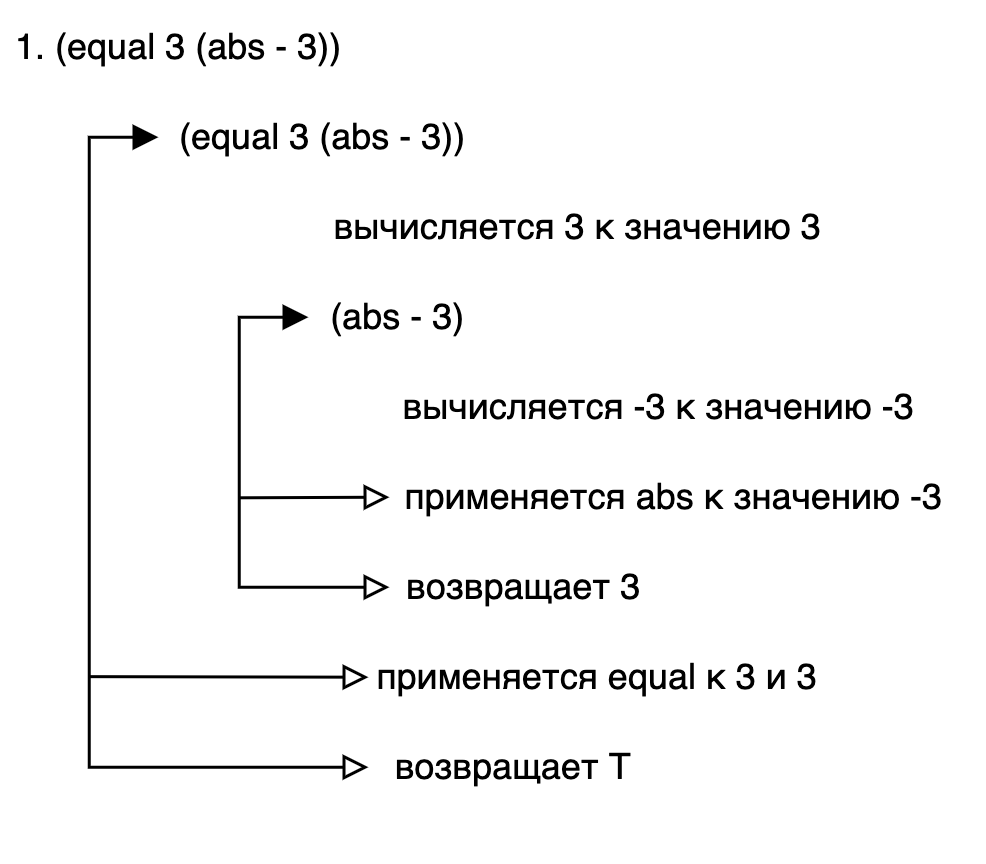
\includegraphics[scale=0.6,left]{task1.1}
%\end{figure}

%\begin{lstinputlisting}[
%	caption={Задание 2},
%	label={lst:t2},
%	style={lsp},
%	linerange={3-4},
%	]{../src/main.lsp}
%\end{lstinputlisting}

